\subsection{Skalarum}
Objekter i virkeligheden, såvel som detaljer i et billede, optræder kun som meningsfulde enheder over et specifikt skalainterval, bundet af en indre og en ydre skala. Et simpelt eksempel er et træ, der indenfor centimeters eller nanometers afstand vil optræde som blade eller molekyler og indenfor meters afstand, vil opfattes som et træ. Koenderink \cite{koen} definere et objekts skalainterval som værende afgrænset af to skalaer: den inderste og den yderste skala,  F.eks. vil en trætop have en indre skala på ca. 10 cm og en ydre skala på ca. 10 m. 
\\
Formelt kan et billede repræsenteres som en funktion af to variable:
\begin{equation}
\begin{split}
&I: R^2 \rightarrow R \\
&I(x,y) = \lambda \hspace{0.5 cm} (x,y)\in R^2, \lambda \in R
\end{split}
\end{equation}
hvor $\lambda$ repræsentere en billedintensitet. Da billedet indeholder en ukendt scene, vides det ikke hvilket skalainterval, der for et givent objekt indgående i scenen, er meningsfuldt. Den inderste skala af billedet vil derfor være bundet af pixelstørrelsen og den ydre af billedets fysiske størrelse. En aksiomatisk tilgang til dette problem er at undersøge en bred skalarepræsentation af billedet i form af en udvidelse af billedfunktionen med en enkelt parameter også kaldt skalaparametren $\sigma$:
\begin{equation}
\begin{split}
&L: R^3 \rightarrow R \\
&L(x,y,\sigma) = \lambda \hspace{0.5 cm} (x,y,\sigma)\in R^3, \lambda \in R
\end{split}
\end{equation}
For at opnå en multi-skal repræsentation af billedet, oprettes der et skalarum bestående af skalabilleder, der går fra at udtrykke finere til grovere strukturer, proportionelt med skalaparametren, som illustreret i figur \ref{fig:scalerep}. 
\begin{figure}[H]
    \centering
    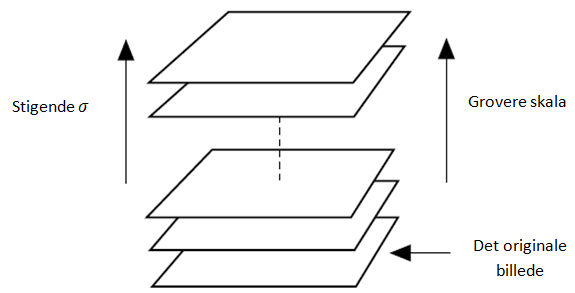
\includegraphics[width=0.45\textwidth]{fig/32.png}
     \vspace{-1em}
    \begin{center}    
       \caption{\textcolor{gray}{\footnotesize \textit{ }}}
    \label{fig:scalerep}
     \end{center}
     \vspace{-2.5em}
  \end{figure} \noindent
Denne overgang fra finere til grovere strukturer kan opnås ved iterativt at folde billederne med et Gaussisk filter af stigende $\sigma$ værdi, hvor billedets nulskala repræsenteres ved biledet $ L(x,y,0) = I(x,y)$ og for $\sigma>0$:
\begin{equation}
L(x,y,\sigma) = G(x,y,\sigma)\ast I(x,y)
\label{scalespace1}
\end{equation}
\\
Der anvendes et Gaussisk filter, på grund af dens unikke egenskaber,  bl.a. at der ikke forekommer nye strukturer ved glatning, når skalaparametren stiger. Glatningen af billedet kan ses som at billedet flades ud og derved vil intensiteten i maksima falde og stige i minima.  Witkins \cite{witkins} beviste dette i tilfældet for én-dimensionselle signaler illustreret i  figur  \ref{scalespace1}, der viser resultatet af at glatte et signal med et Gaussisk filter af stigende $\sigma$ værdi. Det ses tydeligt, hvordan signalets underliggende grovere struktur bliver udtrykt og at finere strukturer undertrykkes.
\begin{figure}[H]
    \centering
    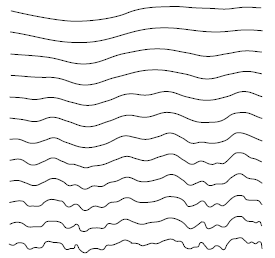
\includegraphics[width=0.45\textwidth]{fig/33.png}
     \vspace{-1em}
    \begin{center}    
       \caption{\textcolor{gray}{\footnotesize \textit{ }}}
    \label{fig:scalereps}
     \end{center}
     \vspace{-2.5em}
  \end{figure} \noindent
Koenderink \cite{koen} førte dette begreb videre til det to-dimensionelle tilfælde, ved at vise at foldningen af billedet med et Gaussisk filter er den generelle løsning til diffusionsligningen, som beskriver hvordan en varmefordeling $I$ udvikler sig over tid $t$.
$$ \partial t I = \nabla^2I $$
\subsection{Skala Pyramide}
En måde, at repræsentere et skalrum er ved en \textit{skalapyramide}. En skalapyramide repræsentation er en datatype, der opretter en række kopier af et billede, der iterativt reduceres i størrelse. Imellem, hvert nivuaeu af pyramiden er billedet foldet med et Guassisk filter og derefter halveret i størrelsen.
\begin{figure}[H]
    \centering
    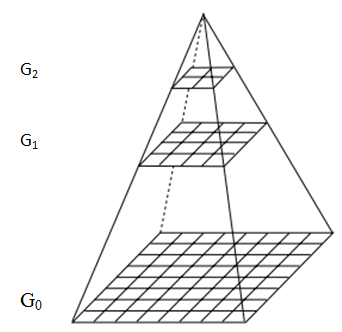
\includegraphics[width=0.40\textwidth]{fig/40.png}
     \vspace{-1em}
    \begin{center}    
       \caption{\textcolor{gray}{\footnotesize \textit{ }}}
    \label{fig:scalerepdiff}
     \end{center}
     \vspace{-2.5em}
  \end{figure} \noindent
Hvis $REDUCE$ betegner operatoren der reducere billedet og $G$ er skalapyramide repræsentation, hvor $G_0$ er det originale billede, kan de forskellige niveauer opnås ved:
\begin{equation}
G_l =REDUCE[G_{l-1}]
\end{equation}
Nærmere kan operationen beskrives som:
\begin{equation}
G_l(i,j)=\sum\limits_{m}\sum\limits_{n}w(m,n)G_{l-1}(2i+m,2j+n)
\end{equation}
hvor $w$ er et Gaussisk filter. Figur \ref{fig:scalerepdiff} viser sammenhængen med at (a) anvende et Gaussisk filter af iterativt stigende størrelse, og (b) ved at oprette en skalapyramide.
\begin{figure}[H]
    \centering
    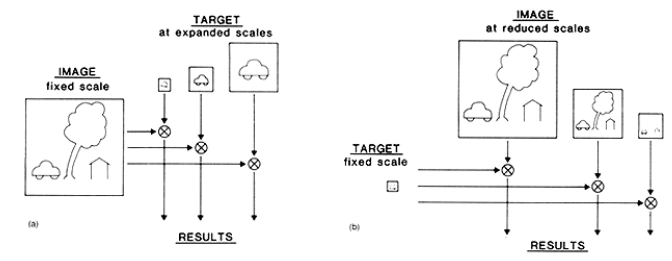
\includegraphics[width=0.90\textwidth]{fig/38.png}
     \vspace{-1em}
    \begin{center}    
       \caption{\textcolor{gray}{\footnotesize \textit{ }}}
    \label{fig:scalerepdiff}
     \end{center}
     \vspace{-2.5em}
  \end{figure} \noindent
Fordelene ved en pyramide repræsentation er at  billedernes størrelser reduceres, hvilket reducere antallet af beregninger drastisk.